\documentclass[12pt]{article}

\usepackage{sbc-template} 
\usepackage{graphicx,url}
\usepackage{url}
\usepackage[brazil]{babel} 
\usepackage[utf8]{inputenc} 
\usepackage[T1]{fontenc}
\usepackage[normalem]{ulem}
\usepackage[hidelinks]{hyperref}

\usepackage[square,authoryear]{natbib}
\usepackage{amssymb} 
\usepackage{mathalfa} 
\usepackage{algorithm} 
\usepackage{algpseudocode} 
\usepackage[table]{xcolor}
\usepackage{array}
\usepackage{titlesec}
\usepackage{mdframed}
\usepackage{listings}
\usepackage{hyperref} 
\usepackage{amsmath} 
\usepackage{booktabs}

\urlstyle{same}

\newcolumntype{L}[1]{>{\raggedright\let\newline\\\arraybackslash\hspace{0pt}}m{#1}}
\newcolumntype{C}[1]{>{\centering\let\newline\\\arraybackslash\hspace{0pt}}m{#1}}
\newcolumntype{R}[1]{>{\raggedleft\let\newline\\\arraybackslash\hspace{0pt}}m{#1}}

\newcommand\Tstrut{\rule{0pt}{2.6ex}} 
\newcommand\Bstrut{\rule[-0.9ex]{0pt}{0pt}} 
\newcommand{\scell}[2][c]{\begin{tabular}[#1]{@{}c@{}}#2\end{tabular}}

\usepackage[nolist,nohyperlinks]{acronym}

\title{Infraestrutura de Hardware - IF674}

\author{Amanda Arruda Melo Silva\inst{1}}


\address{Universidade Federal de Pernambuco - UFPE
	\email{aams2@cin.ufpe.br}
}

\begin{document} 
	
	\maketitle
	
	\begin{resumo} 
	    A disciplina de Infraestrutura de Hardware é ofertada aos alunos do terceiro período do curso de Ciência da Computação, lecionada pelo professor Adriano Sarmento, que visa apresentar um panorama a respeito dos componentes de um sistema computacional.

	\end{resumo}
	
	\section{Introdução}
	\label{sec:introducao}
	
        O objetivo do curso é ministrar aos alunos um conteúdo capaz de transmitir uma visão geral a respeito dos componentes físicos presentes em computadores, com um maior enfoque em transmitir os princípios desses aparelhos.
    	
    	A partir disso, os alunos poderão aliar o entendimento teórico à prática por meio de projetos de versões físicais mais simples ou ferramentas de simulação das peças estudadas. Também serão trabalhados conceitos mais elevados, como as técnicas utilizadas nos processadores mais reccentes a fim de aumentar o desempenho dos computadores, como super-escalares e pipeline.
    	
    	Outros tópicos abordados envolvem as principais tecnologias de memória, desempenho dos sistemas computacionais e ainda análises quantitativas a respeito da dependência dos dispositivos de Entrada e Saída.
    	
    	Por fim, a avaliação da disciplina consiste na realização de duas listas, duas avaliações e um projeto, e os conteúdos minsitrados têm como base o livro texto \emph{Organização e Projeto de Computadores: A interface Hardware/Software - David Patterson e John Hennessy.}
    	
        \begin{figure}[!h]
         \centering
         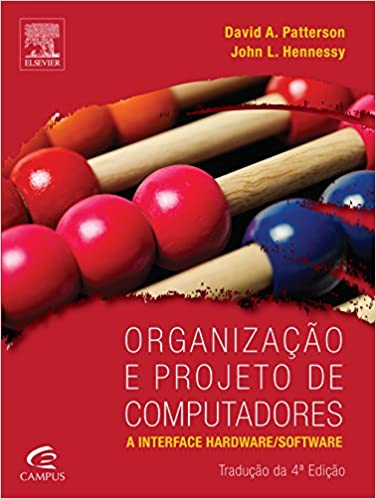
\includegraphics[width=0.3\textwidth]{figures/livro.jpg}
         \caption{Livro texto \citep{CInWiki}}
         \label{fig:livro}
        \end{figure}


	\section{Relevância}
	\label{sec:relevancia}
	
	    Seguindo a metodologia previamente apresentada, o entendimento a respeito dos mais diversos aspectos dos projetos e implementação de computadores vida  auxiliar a vida profissional, formando um cientista da computação capaz de escolher as melhores estratégias para agilizar e aumentar a eficiência da infraestrutura de TI em seu ambiente de trabalho.
	    
	    Ainda sobre o papel fundamental do entendimento do software, vale ressaltar o alerta feito por David. A Patterson: \emph{"Nossa visão é que, pelo menos na próxima década, a maioria dos programadores terá de entender a interface hardware/software se quiser que os programas executem de modo eficiente em computadores paralelos."}\citep{organizacao_projeto}
	    
        \begin{figure}[!h]
         \centering
         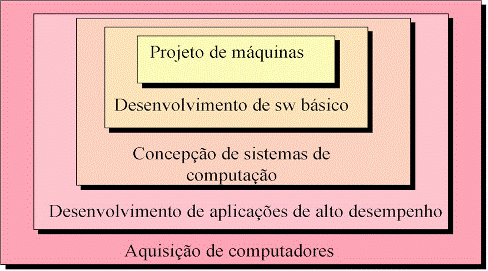
\includegraphics[width=0.6\textwidth]{figures/aplicacoes.png}
         \caption{Aplicações práticas da disciplina \citep{IF674}}
         \label{fig:aplicacoes}
        \end{figure}

	\section{Relação com outras disciplinas}
	\label{sec:relacao}
	
        A disciplina possui dois pré-requisitos. São eles: Introdução à Programação - IF699, cursado no primeiro período, e Sistemas Digitais - IF675, cursado no segundo período. Ambas as cadeiras emabasam importantes conceitos de computação úteis para o entendimento dos fundamentos dos componentes estudados e as suas aplicações nos softwares utilizados.
	
    \bibliographystyle{apalike}
	\bibliography{references}
	
\end{document}
